\section{Numerical and Empirical Properties}

\subsection{Approximation of Sum of 2 IID RVs}\label{subsec:convolfit}
Although the convolution of two iid Sinusoidal RVs is not theoretically a \sindist{}, we found that some candidate \sindist{} can often provide good approximation to the same. We may call this phenomenon \textbf{approximate iid stability}. This is an intuitive desideratum in a linear modelling context, where we would want the sum of residuals to (at least approximately) lie in the same distribution family as the individual residuals.

The following computational study is conducted in this regard. Each convolution of the same 2 $\Sinu(s,k)$ densities over grid of $s, k \in (0,2]$ is attempted to be approximated by some candidate $\Sinu(0,2, s^*, k^*)$, by the mode matching algorithm specified in \autoref{sec:modematch}. The reason for choosing $a=0,d=2$ follows heuristically: we expand the support so as to at least contain all values of the sum of the RVs. Hence we attempt the following approximation:

\begin{equation}\Sinu(s,k) * \Sinu(s,k) \approx \Sinu(0, 2, s^*, k^*)\end{equation}\label{eq:locscaleReadj}
for some optimal $s^*$ and $k^*$.

The results of this approximation routine are presented in the form of a heatmap in \autoref{fig:convolfit1}. A poor fit (larger Hellinger distance) appears redder in the plot, whereas a good fit (smaller Hellinger distance) appears greener. Note that the scale is negative logarithmic, i.e. it plots the values of $-\log_{10} (\text{Hellinger distance})$ in colour. Information about the best fitting $s^*, k^*$ are omitted from the plot.

\begin{figure}[h!]
	\centering
	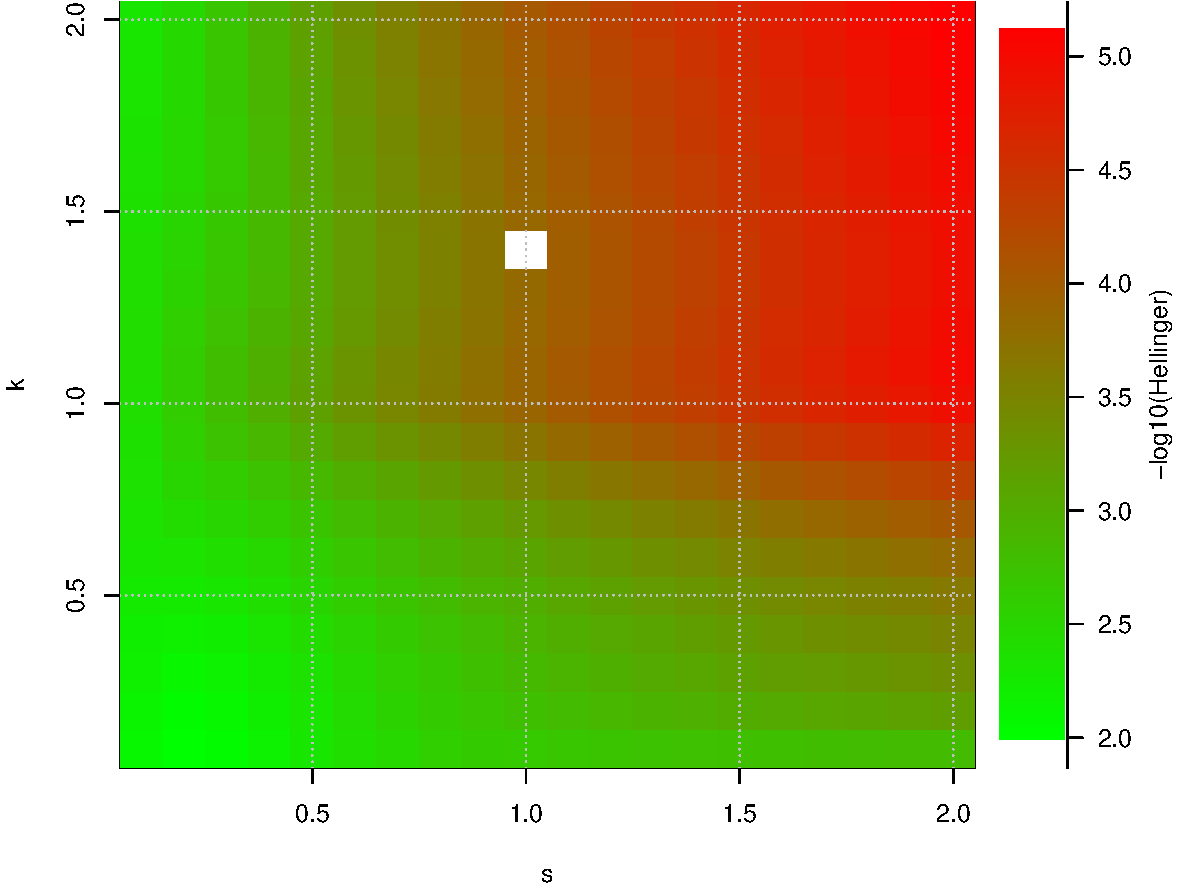
\includegraphics[width=0.6\linewidth]{fig/2.5-sumdens}
	\caption{Different combinations of $(s,k)$ and the degree of approximability (measured wrt. Hellinger distance) of the self-convoluted $\Sinu(s,k)$ density. A greener tone indicates better approximability. The whitened-out pixels came from garbage values (negative, due to computational limitations), probably because such distributions were completely stable!}
	\label{fig:convolfit1}
\end{figure}

\subsection{Skewness-Kurtosis cover}
Choosing the standard $\Sinu(s,k)$ family, we analyze its skewness-kurtosis cover in \autoref{fig:skewkurtcover} over a finite grid of parameter choices: $s,k = 0.05\,(0.05)\, 6$. The plot is colorized to indicate the choice of parameters as denoted in the legend aside.

\begin{figure}[h!]
	\centering
	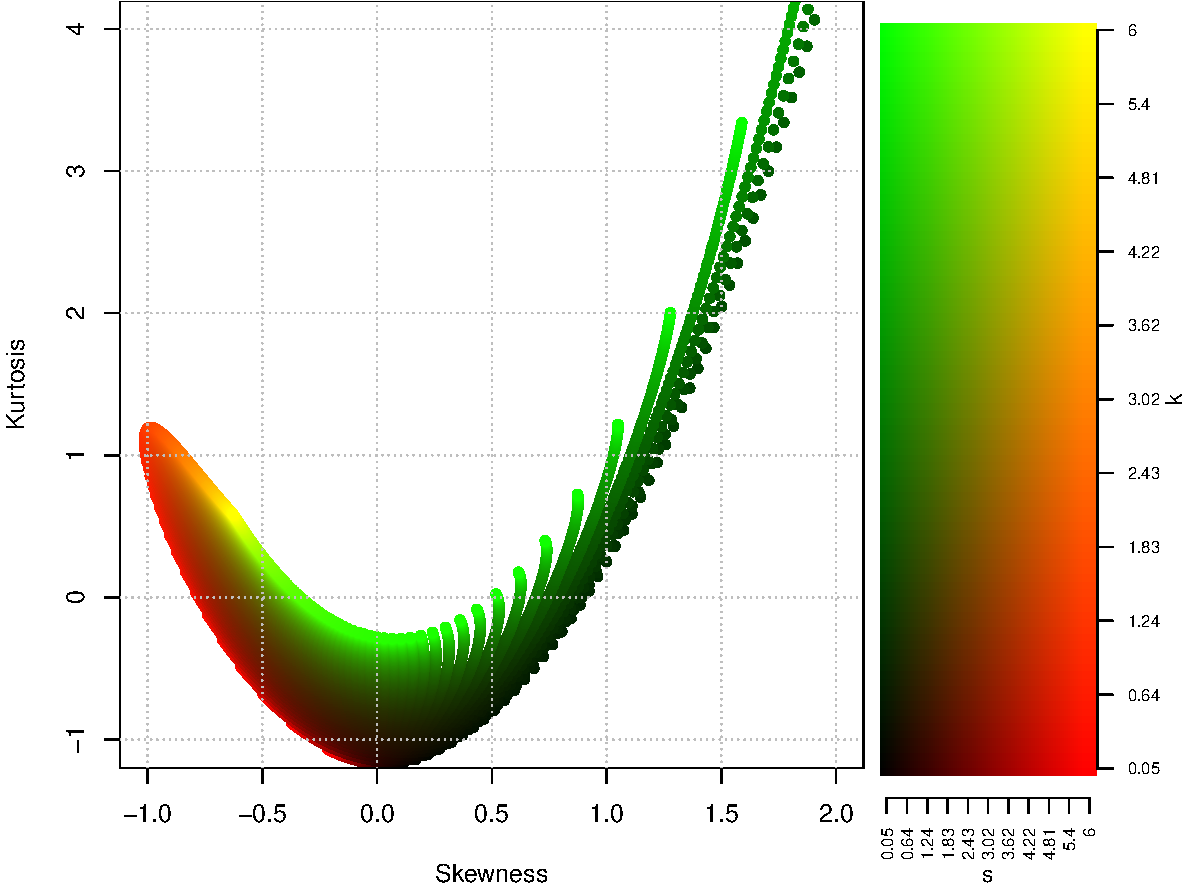
\includegraphics[width=0.8\linewidth]{fig/2-skewkurtcover}
	\caption{Skewness-Kurtosis cover of the \sindist.}
	\label{fig:skewkurtcover}
\end{figure}
